\begin{longtable}{l|X|X|X}
\toprule
\multicolumn{4}{c}{Classical Games (\ding{182} last one wins (normal); \ding{183} last one loses (mis\`ere))} \\ \hline
Name & Description & Criteria / Opt.strategy & Remarks \\ \hline

NIM & $n$ piles of objs. One can take any number of objs from any pile (i.e. set of possible moves for the $i$-th pile is $M=[pile_i]$, $[x]:=\{1,2,...,\lfloor x \rfloor\}$).  & $SG=\otimes_{i=1}^n pile_i$. Strategy: \ding{182} make the Nim-Sum 0 by \emph{decreasing} a heap; \ding{183} the same, except when the normal move would only leave heaps of size 1. In that case, leave an odd number of 1's. & The result of \ding{183} is the same as \ding{182}, opposite if all piles are 1's. Many games are essentially NIM.\\ \hline

NIM (powers) & $M = \{a^m|m\ge 0\}$& If $a$ odd:\newline $SG_n = n \% 2$ & If $a$ even:\newline $SG_n = 2$, if $n\equiv a\%(a+1)$;\newline $SG_n = n \% (a+1) \% 2$, else.  \\ \hline

NIM (half) & $M_{\text{\ding{172}}} = [\frac{pile_i}{2}]$\newline $M_{\text{\ding{173}}} = [\lceil \frac{pile_i}{2} \rceil\text{, } pile_i]$ & \ding{172}$SG_{2n} = n$, $SG_{2n+1}=SG_{n}$\newline \ding{173}$SG_0=0$, $SG_n=[\log_2 n]+1$  & \\ \hline

NIM (divisors)&$M_{\text{\ding{172}}} = \text{divisors of } pile_i$\newline $M_{\text{\ding{173}}} = \text{proper divisors of }pile_i$ & \ding{172}$SG_0 = 0$, $SG_n = SG_{\text{\ding{173}},n} + 1$ \newline \ding{173}$SG_1=0$, $SG_n=$ number of 0's at the end of $n_{binary}$ \\ \hline

Subtraction Game & $M_{\text{\ding{172}}} = [k]$\newline $M_{\text{\ding{173}}} = S$ (finite)\newline $M_{\text{\ding{174}}} = S \cup \{pile_i\}$ & $SG_{\text{\ding{172}},n} = n \mod (k+1)$. \ding{182}lose if $SG=0$; \ding{183}lose if $SG=1$. $SG_{\text{\ding{174}},n} = SG_{\text{\ding{173}},n}+1$ & For any finite $M$, $SG$ of one pile is eventually periodic.\\ \hline

Moore's NIM$_k$ & One can take any number of objs from at most k piles. & \ding{182}Write $pile_i$ in binary, sum up in base $k+1$ without carry. Losing if the result is 0. & \ding{183} If all piles are 1's, losing iff $n\equiv 1\%(k+1)$. Otherwise the result is the same as \ding{182}. \\ \hline

Staircase NIM & $n$ piles in a line. One can take any number of objs from $pile_i$, $i>0$ to $pile_{i-1}$ & Losing if the NIM formed by the odd-indexed piles is losing(i.e. $\otimes_{i=0}^{(n-1)/2} pile_{2i+1}=0$)\\ \hline

Lasker's NIM & Two possible moves: 1.take any number of objs; 2.split a pile into two (no obj removed) & $SG_n = n, \text{ if }n\equiv 1,2(\% 4)$\newline $SG_n = n+1, \text{ if }n\equiv3(\% 4)$\newline $SG_n = n-1, \text{ if }n\equiv0(\% 4)$ \\ \hline

Kayles & Two possible moves: 1.take 1 or 2 objs; 2.split a pile into two (after removing objs) & $SG_n$ for small $n$ can be computed recursively. $SG_n$ for $n \in [72,83]$: 4 1 2 8 1 4 7 2 1 8 2 7 & $SG_n$ becomes periodic from the 72-th item with period length 12.  \\ \hline

Dawson's Chess& $n$ boxes in a line. One can occupy a box if its neighbours are not occupied. & $SG_n$ for $n\in [1,18]$: 1 1 2 0 3 1 1 0 3 3 2 2 4 0 5 2 2 3 & Period = 34 from the 52-th item.\\ \hline

Wythoff's Game& \textbf{Two} piles of objs. One can take any number of objs from either pile, or take the \emph{same} number from \emph{both} piles.&$n_k = \lfloor k \phi \rfloor = \lfloor m_k \phi \rfloor -m_k$ \newline $m_k = \lfloor k \phi^2 \rfloor = \lceil n_k \phi \rceil = n_k + k$ \newline $\phi:=\frac{1+\sqrt{5}}{2}$. $(n_k,m_k)$ is the $k$-th losing position. & $n_k$ and $m_k$ form a pair of complementary Beatty Sequences (since$\frac{1}{\phi}+\frac{1}{\phi^2}=1$). Every $x>0$ appears either in $n_k$ or in $m_k$.\\ \hline

Mock Turtles & $n$ coins in a line. One can turn over 1, 2 or 3 coins, with the rightmost from head to tail. & $SG_n = 2n$, if $\mathrm{ones}(2n)$ odd; $SG_n = 2n + 1$, else. $\mathrm{ones}(x)$: the number of 1's in $x_{binary}$ & $SG_n$ for $n\in [0,10]$ (leftmost position is 0): 1 2 4 7 8 11 13 14 16 19 21 \\ \hline

Ruler & $n$ coins in a line. One can turn over any \emph{consecutive} coins, with the rightmost from head to tail. & $SG_n=$ the largest power of 2 dividing $n$. This is implemented as $n$\&$-n$(lowbit) & $SG_n$ for $n\in [1,10]$: 1 2 1 4 1 2 1 8 1 2\\ \hline

Hackenbush-tree & Given a forest of rooted trees, one can take an edge and remove the part which becomes unrooted. & At every branch, one can replace the branches by a non-branching stalk of length equal to their nim-sum. & \vtop{\vskip0pt \hbox{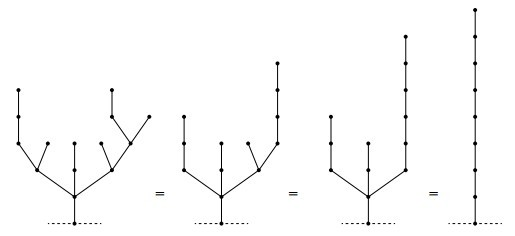
\includegraphics[width=4.5cm]{Formulae_gametheory_hackenbush_colon.jpg}}}\\ \hline

Hackenbush-graph & \vtop{\vskip0pt \hbox{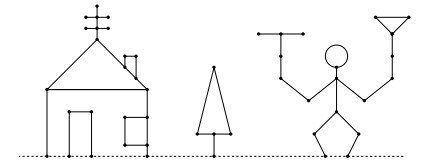
\includegraphics[width=4.5cm]{Formulae_gametheory_hackenbush_graph_example.jpg}}} & Vertices on any circuit can be \emph{fused} without changing SG of the graph. Fusion: two neighbouring vertices into one, and bend the edge into a loop. & \vtop{\vskip0pt \hbox{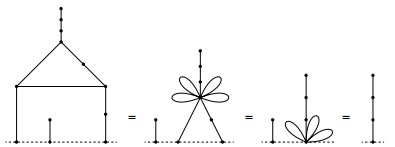
\includegraphics[width=4.5cm]{Formulae_gametheory_hackenbush_graph_fusion.jpg}}}\\

\bottomrule
\end{longtable}